\documentclass{bioinfo}
\usepackage{hyperref}

\copyrightyear{2015}
\pubyear{2015}

\begin{document}
\firstpage{1}

\title[BRAKER1]{BRAKER1: Unsupervised RNA-Seq-Based Genome Annotation with GeneMark-ET and AUGUSTUS}
\author[Hoff \textit{et~al}]{Katharina J. Hoff\,$^{1}$\footnote{to whom correspondence should be addressed}, Simone Lange\,$^{1}$, Alexandre Lomsadze\,$^{2}$, Mark Borodovsky\,$^{2,3,4,5}$ and Mario Stanke\,$^1$}
\address{$^{1}$Ernst Moritz Arndt Universit\"{a}t Greifswald, Institute for Mathematics and Computer Science, Walther-Rathenau-Stra\ss{}e 47, 17487 Greifswald, Germany\\
$^{2}$School of Computational Science and Engineering\\
$^{3}$Center for Bioinformatics and Computational Genomics, Georgia Institute of Technology, Atlanta, GA 30332, USA\\
$^{4}$Department of Biological and Medical Physics, Moscow Institute of Physics and Technology, Dolgoprudny, Moscow Region, Russia\\
$^{5}$Joint Georgia Tech and Emory University Wallace H Coulter Department of Biomedical Engineering, Atlanta, GA 30332, USA}

\history{Received on XXXXX; revised on XXXXX; accepted on XXXXX}

\editor{Associate Editor: XXXXXXX}

\maketitle

\begin{abstract}

\section{Motivation:}

GeneMark-ET is a gene prediction tool that incorporates unassembled RNA-Seq reads into unsupervised training and subsequently generates \textit{ab initio} gene predictions. AUGUSTUS is a gene finder that usually requires supervised training and uses information form unassembled RNA-Seq reads in the prediction step. 

\section{Results:}
We present BRAKER1, a pipeline for unsupervised RNA-Seq-based genome annotation that combines the advantages of GeneMark-ET and AUGUSTUS. BRAKER1 requires an RNA-Seq read alignment file and a genome file as input. First, GeneMark-ET performs iternative training and generates initial gene structures. Second, AUGUSTUS uses predicted genes for training and then integrates RNA-Seq read information into final gene predictions. In our experiments, we observed that BRAKER1 was more accurate than MAKER2 when it is using RNA-Seq as sole source for training and prediction. BRAKER1 does not require pre-trained parameters or a separate training step.

\section{Availability:}
BRAKER1 is available for download at \url{http://bioinf.uni-greifswald.de/downloads/} and \url{http://exon.gatech.edu/.}.

\section{Contact:} \href{katharina.hoff@uni-greifswald.de}{katharina.hoff@uni-greifswald.de}
\end{abstract}

\section{Introduction}



Today, many genome sequencing projects are accompanied by high throughput transcriptome sequencing (RNA-Seq). RNA-Seq can aid the structural annotation of (highly) expressed protein coding genes. The RGASP

Structural gene prediction is an important step in the analysis of sequenced genomes because downstream analysis depends on accurate prediction. Many genome sequencing projects are accompanied by transcriptome sequencing. Transcriptome sequencing can aid structural genome annotation with tools that rely on statistical models. Such tools usually require a training step to adapt species specific parameters. With few exceptions, a previously existing set of reliable genes is required for training (e.g.~generated from ESTs or protein to genome alignments). Since large scale transcriptome sequencing became available, it has been tried to gene finders on assembled RNA-Seq data [cite MAKER2 here?]. Assembled RNA-Seq has also been used to improve gene prediction after training. However, transcriptome assembly is prone to errors, and using such erroroneus data for training and prediction bears the risk of transferring errors into structural genome annotation [check what GeneMark-ET paper cited for this]. If raw read mappings are used instead of assembled transcripts, this problem is avoided.

GeneMark-ET is a gene prediction tool that incorporates unassembled RNA-Seq reads into unsupervised training and subsequently generates \textit{ab initio} gene predictions. 




\begin{methods}
\section{Pipeline Description}

BRAKER1 is implemented in Perl and requires two input files: an RNA-Seq alignment file in \texttt{bam}-format, and a corresponding genome file in \texttt{fasta}-format. Spliced alignment information is extracted from the RNA-Seq file and stored in \texttt{gff}-format. GeneMark-ET uses the genome file and  the spliced alignment \texttt{gff}-file for RNA-Seq supported unsupervised training. After training, GeneMark-ET creates an \textit{ab initio} gene set. Those gene structures that have support by RNA-Seq alignments in all introns are selected for automated training of AUGUSTUS. After training, AUGUSTUS predicts genes in the intput genome file using spliced alignment information from RNA-Seq as extrinsic evidence. The pipeline is illustrated in figure \ref{pipeline}.

\begin{figure}[!tpb]%figure1
\centerline{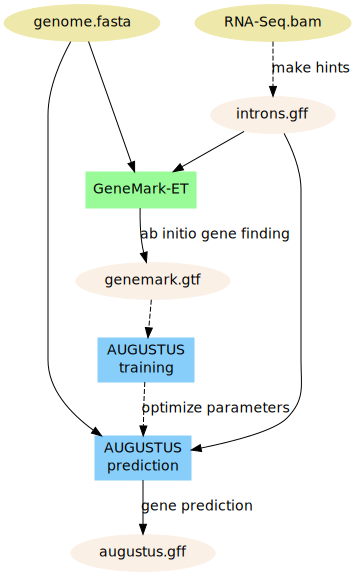
\includegraphics[width=0.6\linewidth]{figs/simple_braker.pdf}}
\caption{Schematic view of the BRAKER1 pipeline.}\label{pipeline}
\end{figure}

\begin{table*}[!t]
\processtable{Accuracy results of BRAKER1 and MAKER2 in genomes of four model organisms. For BRAKER1, accuracy is shown for the GeneMark-ET \textit{ab initio} predictions as well as for the AUGUSTUS predictions with hints from RNA-Seq.\label{Tab:01}}
{\begin{tabular}{lp{.9cm}p{.9cm}p{.9cm}p{.9cm}p{.9cm}p{.9cm}p{.9cm}p{.9cm}p{.9cm}p{.9cm}p{.9cm}p{.9cm}}\toprule
 & \multicolumn{3}{c}{\textit{Arabidopsis thaliana}} &  \multicolumn{3}{c}{\textit{Caenorhabditis elegans}} &  \multicolumn{3}{c}{\textit{Drosophila melanogaster}} &  \multicolumn{3}{c}{\textit{Schizosaccharomyces pombe}}\\
 & \tiny{BRAKER1-GeneMark} & \tiny{BRAKER1-AUGUSTUS} & \tiny{MAKER2} & \tiny{BRAKER1-GeneMark} & \tiny{BRAKER1-AUGUSTUS} & \tiny{MAKER2} & \tiny{BRAKER1-GeneMark} & \tiny{BRAKER1-AUGUSTUS} & \tiny{MAKER2} & \tiny{BRAKER1-GeneMark} &\tiny{BRAKER1-AUGUSTUS} & \tiny{MAKER2}\\
 \midrule
Gene sensitivity & 53.9 & 63.2 & 51.3 & 43.0 & 55.1& 41.0 & 58.5& 70.23 & 58.0 & 80.0& 77.3  & 42.7\\
Gene specificity & 46.1 & 51.3 & 52.5& 41.7& 56.1& 30.8& 49.9 & 59.0 & 46.9& 84.9& 81.2& 68.6\\
Transcript sensitivity & 45.4 & 53.9 & 43.5& 32.9& 43.2& 31.3& 42.3 &52.0 & 42.3 & 80.0& 77.3& 42.7\\
Transcript specificity & 46.1 & 50.0 & 52.5& 41.7 & 54.0& 30.8 & 49.9 & 57.8 & 47.9 &84.9 & 77.4 & 68.6\\
Exon sensitivity & 81.1 & 83.0 & 76.1& 79.9& 80.9& 69.4 & 68.5& 75.1& 64.9& 85.2 & 84.2 & 50.1 \\
Exon specificity & 72.4 & 78.5 & 76.1& 78.2& 85.4& 62.3 & 57.9 & 66.2 & 55.0 & 89.0& 82.6& 71.4\\
\botrule

\end{tabular}}{}
\end{table*}

\section{Test Data}

In order to demonstrate prediction accuracy, genomes, reference annotations and RNA-Seq libraries were retrieved for four model organisms from the respective databases: for \textit{Arabidopsis thaliana}, TAIR 10 was downloaded from http://arabidopsis.org/; for \textit{Caenorhabditis elegans}, WS240 was downloaded from http://www.wormbase.org/; for \textit{Drosophila melanogaster}, R5 was downloaded from http://flybase.org/; for \textit{Schizosaccharomyces pombe}, ASM294v2.23 was downloaded from http://www.pombase.org/. The following RNA-Seq libraries were retrieved from the short read archive at NCBI: SRR934391 (for \textit{A.~thaliana}); SRR065719 (for \textit{C.~elegans}); SRR023505, SRR023546, SRR023608, SRR026433, SRR027108 (for \textit{D.~melanogaster}); SRR097898, SRR097899, SRR097900, SRR097902, SRR097903,
SRR097905, SRR097906, SRR097907, SRR097908, SRR097909,
SRR097912, SRR097915, SRR097917, SRR097921, SRR097922,
SRR097925, SRR402833 (for \textit{S.~pombe}).



\end{methods}


% 
% \begin{figure}[!tpb]%figure2
% %\centerline{\includegraphics{fig02.eps}}
% \caption{Caption, caption.}\label{fig:02}
% \end{figure}

\section{Accuracy Results}



%%%%%%%%%%%%%%%%%%%%%%%%%%%%%%%%%%%%%%%%%%%%%%%%%%%%%%%%%%%%%%%%%%%%%%%%%%%%%%%%%%%%%
%
%     please remove the " % " symbol from \centerline{\includegraphics{fig01.eps}}
%     as it may ignore the figures.
%
%%%%%%%%%%%%%%%%%%%%%%%%%%%%%%%%%%%%%%%%%%%%%%%%%%%%%%%%%%%%%%%%%%%%%%%%%%%%%%%%%%%%%%






\section{Conclusion}


\section*{Acknowledgement}

We would like to thank Mark Yandell and Carson Holt for valuable advice on running MAKER2.

\paragraph{Funding\textcolon} This work is supported by the US National Institutes of Health grant HG000783.

%\bibliographystyle{natbib}
%\bibliographystyle{achemnat}
%\bibliographystyle{plainnat}
%\bibliographystyle{abbrv}
%\bibliographystyle{bioinformatics}
%
%\bibliographystyle{plain}
%
%\bibliography{Document}


\begin{thebibliography}{}
\bibitem[Steijger {\it et~al}., 2013]{RGASP} Steijger,T. and Abril,J.F. and Engstr\"{o}m,P.G. and Kokocinski,F. and The RGASP Consortium, Hubard,T.J. and Guigo,R. and Harrow, J. and Bertone, P. (2013) Assessment of transcript reconstruction methods for
 RNA-seq, {\it Nature Methods}, doi:10.1038/nmeth.271.

\bibitem[Lomsadze {\it et~al}., 2014]{GeneMark-ET} Lomsadze, A. and Burns, P.D. and Borodovsky, M. (2014) Integration of mapped RNA-Seq reads into automatic training of eukaryotic gene finding algorithm, {\it Nucleic Acids Research}, doi:10.1093/nar/gku557.

\bibitem[Stanke \textit{et~al}., 2008]{AUGUSTUS}
Stanke, M. and Diekhans, M. and Baertsch, R. and Haussler, D. (2008) Using native and syntenically mapped cDNA alignments to improve de novo gene finding, \textit{Bioinformatics}, \textbf{24}(5), 637.


\end{thebibliography}
\end{document}
